\documentclass[border=8pt]{standalone}
\usepackage{fontspec}\usepackage{tikz}
\usetikzlibrary{arrows.meta,positioning}
\definecolor{NouOrange}{HTML}{FA4D1F}\definecolor{NouBlack}{HTML}{000000}
\begin{document}
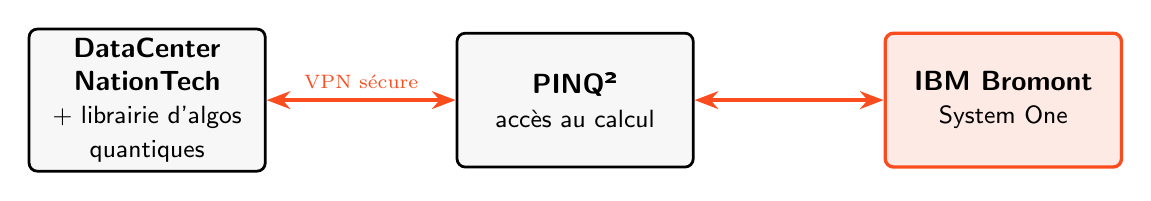
\begin{tikzpicture}[font=\sffamily,
  b/.style={draw=NouBlack,line width=1pt,rounded corners=3pt,align=center,minimum width=3cm,minimum height=1.7cm,fill=black!3}]
  \node[b] (dc) {\textbf{DataCenter}\\\textbf{NationTech}\\{\small + librairie d'algos}\\{\small quantiques}};
  \node[b,right=2.4cm of dc] (pinq) {\textbf{PINQ²}\\{\small accès au calcul}};
  \node[b,right=2.4cm of pinq,fill=NouOrange!12,draw=NouOrange,line width=1.2pt] (ibm) {\textbf{IBM Bromont}\\{\small System One}};
  \draw[{Stealth[length=3mm]}-{Stealth[length=3mm]},NouOrange,line width=1.4pt] (dc) -- node[above,font=\scriptsize]{VPN sécure}(pinq);
  \draw[{Stealth[length=3mm]}-{Stealth[length=3mm]},NouOrange,line width=1.4pt] (pinq) -- (ibm);
\end{tikzpicture}
\end{document}
